\documentclass[UTF8]{ctexart}

\usepackage{anyfontsize}
\usepackage{geometry}
    \geometry{left=4cm,right=4cm,top=2cm,bottom=2cm}
\usepackage{amsmath, amssymb, amsthm}
    \newtheorem{definition}{Definition}
    \newtheorem{theorem}{Theorem}
\usepackage{caption} 	 % 标题
\usepackage{xcolor} 	 % 颜色
\usepackage{graphicx} 	 % 引用图片
\usepackage{float}
\usepackage{framed} 	 % 方框 \begin{framed}
\usepackage{tcolorbox}
    \newtcolorbox{defbox}{colback = blue!20!green!10!white}
    \newtcolorbox{thmbox}{colback = cyan!10!white}
\usepackage{indentfirst} 	 % 首行缩进 
    \setlength{\parindent}{0em}
\usepackage{setspace} 	 % 行间距 \begin{spacing}{arg}
\usepackage{extarrows} 	 % 箭头宏包 \xLongrightarrow 
\usepackage{esvect} 	 % 向量箭头 \vv{}
\usepackage{siunitx} 	 % 国际单位 \si{unit} \SI{number}{unit} 
\usepackage{esint} 	 % 积分符号
\usepackage{mathrsfs}
\usepackage{multirow}


% font
\newcommand{\ve}[1]{\boldsymbol{\mathbf{#1}}}
\newcommand{\unit}[1]{\boldsymbol{\mathbf{\hat{#1}}}}
\newcommand{\mr}{\mathrm}
\newcommand{\mcal}{\mathcal}
\newcommand{\mscr}{\mathscr}
% common symbol
\newcommand{\E}{\mathrm e}
\renewcommand{\I}{\mathrm i}
\newcommand{\R}{\mathbb R}
\newcommand{\Z}{\mathbb Z}
\newcommand{\N}{\mathbb N}
\newcommand{\Q}{\mathbb Q}
\newcommand{\C}{\mathbb C}
% differentiation
\def \DD #1.#2.#3 {\dfrac{d^{#1} #2}{d #3^{#1}}}
\def \PP #1.#2.#3 {\dfrac{\partial^{#1} #2}{\partial #3^{#1}}}
\def \dd #1.#2 {\dfrac{d #1}{d #2}}
\def \pp #1.#2 {\dfrac{\partial #1}{\partial #2}} 
\newcommand{\del}{\nabla}
% other
\newcommand{\transp}{^{\top}}
\DeclareMathOperator{\tr}{tr}
\let\Im\relax
\let\Re\relax
\DeclareMathOperator{\Im}{Im}
\DeclareMathOperator{\Re}{Re}

\pagestyle{empty}

\begin{document}
Note: If it leads to no confusion, italic $ i $ and $ e $ are used to represent imaginary unit and natural constant (Euler's number) respectively, instead of roman $ \mr i $ and $ \mr e $.
\section{Complex Number}
\begin{defbox}
    \begin{definition}[imaginary unit]
        Define \textbf{imaginary unit} $ i $ by $ i^2 = -1 $. Which could be written as $ i = \sqrt{-1} $.
    \end{definition}
\end{defbox}

So it's obvious that: for $ n \in \Z^+ $, $ \sqrt{-n} = \sqrt{-1 \cdot n} = \sqrt{-1} \sqrt{n} = \sqrt{n} i $.
\vskip 1em

Example 1: Solve $ x^2 + x + 1 = 0 $.
\vskip 0.5em

Using \textbf{Vieta's formula}, $ x_1 = \dfrac{-1 + \sqrt{1^2 - 4 \times 1 \times 1}}{2 \times 1} = \dfrac{-1 + \sqrt{-3}}{2} = \dfrac{-1 + \sqrt{3} i}{2} $, it's the same that $ x_2 = \dfrac{-1 - \sqrt{3} i}{2} $.
\vskip 1em

Because $ i^2 = -1 $, $ i^3 = i^2 \cdot i = - i $, $ i^4 = i^2 \cdot i^2 = 1 $. This induces the periodic equalities: $ i^{4k} = 1 $, $ i^{4k+1} = i $, $ i^{4k+2} = -1 $, $ i^{4k+3} = -i $, which hold for all integers $ k $.
\vskip 2em

By combining real numbers and imaginary unit. We can expand $ \R $.

\begin{defbox}
    \begin{definition}
        $ z $ is complex number, if it is in the form $ a + b i $, where $ a $ and $ b $ are real numbers. Here $ a $ is called the real part and $ b $ the imaginary part. The two parts are denoted by $ \Re(z) = a $ and $ \Im(z) = b $. The set of all complex numbers is denoted by $ \C $.
    \end{definition}
\end{defbox}

Letting $ b $ in $ a + bi $ equals $ 0 $, we have $ a $, a real number. So we can see that $ \R \subset \C $. A real number can be regarded a The multipication of $ b $ and $ i $, $ b i $ is commutative, therefore $ a + b i $ may be written as $ a + i b $. For example: $ 1 - 2 i $, $ 3 + i 4 $, $ -3 + i (-2) $.

\subsection{Visualization} \label{section1}
Since a complex number $ a + b i $ is identified with an orderd pair $ (a, b) $, we can intepret complex number as a point in a two-dimensional Cartesian plane, with unique coordinates for each complex number and a unique vector pointing to each of them.
\vskip 1em

The plane, which plots vectors and points representing complex numbers, is called \textbf{complex plane} or \textbf{Argand diagram}. A complex plane have two perpendicular axes, real axis and imaginary axis.

\begin{figure}[H]
    \centering
    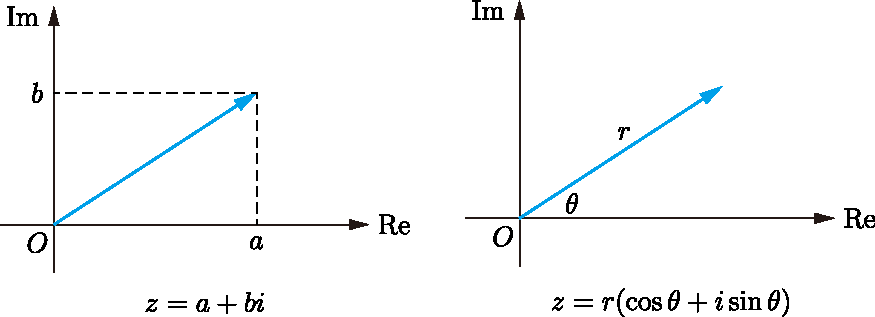
\includegraphics[width = 0.8\linewidth]{./pic/visualization.pdf}
\end{figure}
\vskip 1em

As the figure shows, there're two ways to express a complex number: Cartesian coordinates (left) or polar coordinates (right). $ z = r(\cos\theta + i \sin \theta) $ involves trigonometric function, so it can be called the \textbf{trigonometric form}. 
\vskip 1em

In polar form, $ r $ is called the \textbf{modulus} (length) of the complex number, denoted by $ |z| $; and $ \theta $ is called the \textbf{argument}, denoted by $ \operatorname{Arg} (z) $. 

The two forms have the relation:
\[  
    \begin{cases}
        x = r \cos \theta \\
        y = r \sin \theta
    \end{cases}
    \qquad
    \begin{cases}
        r = \sqrt{x^2 + y^2} \\
        \theta = \arctan \dfrac{y}{x} (\pm \pi)
    \end{cases}
    \,.
\]

To specify the calculation of $ \theta $: when $ x > 0 $, $ \theta = \arctan \dfrac{y}{x} $; when $ x < 0 $ and $ y \geqslant 0 $, $ \theta = \arctan \dfrac{y}{x} + \pi $; when $ x < 0 $ and $ y < 0 $, $ \theta = \arctan \dfrac{y}{x} - \pi $. Also when $ x = 0 $, $ \theta $ is obvious and the formula above is not applicable.

\subsection{Euler's formula} \label{sec2}
Euler's formula declares that: for any $ x \in \R $,
\[ \exp i x = e^{i x} = \cos x + i \sin x \,.\]

This gives us another way two express a complex number:
\[ z = a + b i = r (\cos \theta + i \sin \theta) = r e^{i \theta} \,.\]

\begin{table}[H]
        \centering
        \begin{tabular}{c|c|c}
        \hline
        \multirow{2}{*}{Cartesian form} & \multicolumn{2}{c}{polar form}                                                  \\ \cline{2-3} 
                                        & trigonometric                                  & exponential                     \\ \hline
        \multirow{2}{*}{$a + b i$}      & \multirow{2}{*}{$r(\cos\theta + i\sin\theta)$} & \multirow{2}{*}{$re^{i\theta}$} \\
                                        &                                                &                                 \\ \hline
        \end{tabular}
\end{table}

The three forms are equivalent, and can representing any complex number in complex plane. The conversions among them are given in section \ref{section1}.
\vskip 2em

These are common complex numbers in different forms.
\[ 1 = \exp {i0} \,,\]
\[ i = \exp \left(i\dfrac{\pi}{2}\right) \,.\]
\[ -1 = \exp (i\pi) \,.\]
\[ -i = \exp \left(i\frac{3\pi}{2}\right) \,.\]

And these property are obvious in geometrical view:
\[ re^{i(\theta \pm \pi/2)} = \pm r i e^{i \theta} \,,\]
\[ re^{i(\theta \pm \pi)} = - re^{i\theta} \,.\]


\subsection{Operations and relations}
\subsubsection{Equality}
Two complex number $ z_1 = a_1 + b_1 i $ and $ z_2 = a_2 + b_2 i $ are equal if and only if $ a_1 = a_2 $ meanwhile $ b_1 = b_2 $.

\subsubsection{Addition}
The sum of two complex number is a complex number, which real part and imaginary part is respectively the sum of real parts and the sum of imaginary ones of two complex numbers.
\[ (a + b i) + (c + d i) = (a + c) + (b + d) i  \,.\]

It's convenient to write $ a + b i $ in the form of vector $ (a, b) $, and use the form regarding complex numbers as vectors. 

\[ (a, b) + (c, d) = (a + c, b + d) \,.\]

The visualization of addition of two complex numbers is just like that of two vectors.

\begin{figure}[H]
    \centering
    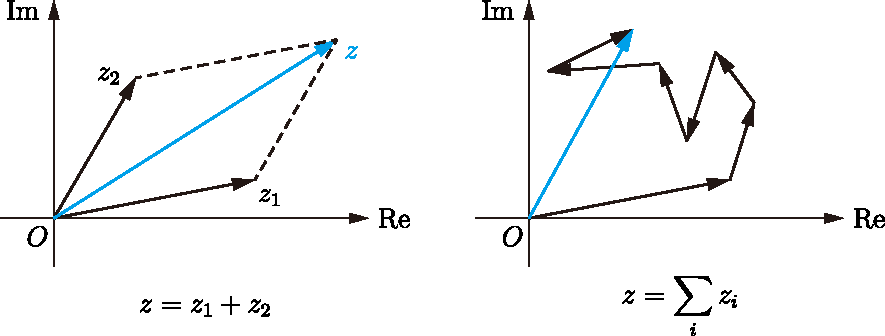
\includegraphics[width = 0.8\linewidth]{./pic/addition.pdf}
\end{figure}



\subsubsection{Multipication}
Under the rules of the distributive property, we can perform:
\[ c \cdot (a + b i) = ca + cb i \,,\]
\[ c \cdot (a, b) = (ca, cb) \,.\]

and the multipication of two complex numbers:
\begin{align*}
    (a + b i) \cdot (c + d i) &= a c + a \cdot d i + b i \cdot c + b i \cdot d i \\
    &= ac + ad i + bc i - bd \\
    &= (ac - bd) + (ad + bc) i \,.
\end{align*}

It will be much more convenient if we use exponential form.

\[ r_1 e^{i \theta_1} \cdot r_2 e^{i \theta_2} = r_1 r_2\, e^{i (\theta_1 + \theta_2)} \,.\]

\begin{figure}[H]
    \centering
    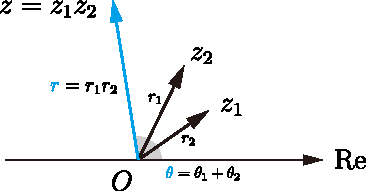
\includegraphics[width = 0.5\linewidth]{./pic/multi.pdf}
\end{figure}

\subsubsection{Subtraction}
With addition and multipication defined, subtraction are easily understood, we can define $ z_1 - z_2 = z_1 + (-1)\cdot z_2 $:
\[ (a, b) - (c, d) = (a - c, b - d) \,,\]

\begin{figure}[H]
    \centering
    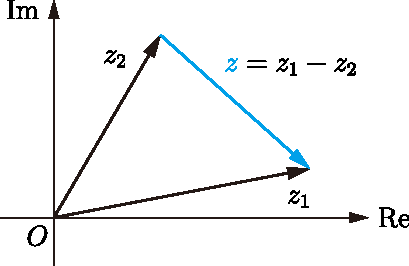
\includegraphics[width = 0.4\linewidth]{./pic/subtraction.pdf}
\end{figure}


These basic operations are very likely the same as real numbers and polynomials. Just use the basic law of  arithmetic operations and notice that $ i^2 = -1 $.

\subsubsection{Rotation} \label{rotation}
We already know from section \ref{sec2} that $ i = e^{i\pi/2} $, so if we multiply a complex number $ z = re^{i\theta} $ by $ i $: $ re^{i\theta} \cdot e^{i\pi/2} = re^{i(\theta + \pi/2)} $. What it leads is the counter-clockwise rotation of original complex number by $ 90^\circ $.
\vskip 1em

\begin{figure}[H]
    \centering
    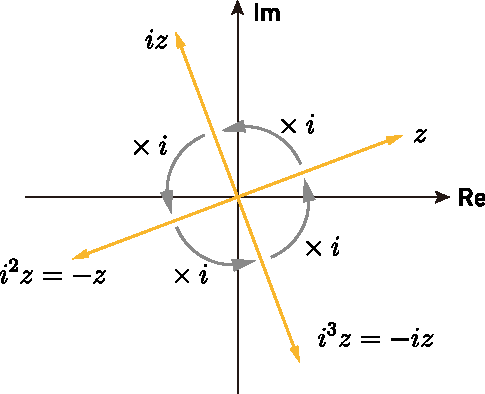
\includegraphics[width = 0.45\linewidth]{./pic/rotate.pdf}
\end{figure}


More generally, if we multiply a complex number $ z $ by another one $ r e^{i \theta} $, we rotate $ z $ counter-clockwise by the angle of $ \theta $ then scale it by $ r $ times.


\subsubsection{Conjugate}
\begin{defbox}
    \begin{definition}
        For $ z = a + b i $, $ a - b i $ is call the (complex) conjugate of $ z $. It's denoted by either $ \bar z $ or $ z^* $.
    \end{definition}
\end{defbox}



Geometrically, \textbf{reflecting a complex number across real axis}, and you will get its conjugate. So when using exponential form, let $ z = r e^{i \theta} $, then $ \bar z = r e^{i(-\theta)} $ is obvious.
\vskip 1em

Let $ z = a + b i $. It's easy to calculate that: \[ z \bar z = a^2 + b^2 = |z|^2 \,.\]

\subsubsection{Reciprocal and division}
Since $ z \bar z = |z|^2 $:
\[ \dfrac{1}{z} = \dfrac{\bar z}{|z|^2} \,.\]

Let $ z = (a, b) $,
\[ \dfrac{1}{z} = \dfrac{\bar z}{|z|^2} = \left( \dfrac{a}{a^2 + b^2}, \dfrac{-b}{a^2 + b^2} \right) \,.\]

Division on complex numbers can be defined by $ z_1 / z_2 = z_1 \cdot z_2^{-1} $. And to look it in another way:

\begin{align*}
    \dfrac{z_1}{z_2} &= \dfrac{z_1 \bar z_2}{z_2 \bar z_2} \\
    & = \dfrac{z_1 \bar z_2}{|z_2|^2}
\end{align*}

Example: $ \dfrac{1 + 2 i}{3 + 4 i} $
\vskip 0.5em
$ \dfrac{1 + 2 i}{3 + 4 i} = \dfrac{(1 + 2i)(3 - 4i)}{(3 + 4i)(3 - 4i)} = \dfrac{11 + 2i}{25} = \dfrac{11}{25} + \dfrac{2}{25} i $.

\vskip 1.5em
Now introducing a special equality:
\[ \dfrac{1}{i} = -i \,.\]

The equality can be explained in two ways. First, $ i = e^{i\pi/2} $, so $ i^{-1} = \left( e^{i \pi/2} \right)^{-1} = e^{i(-\pi/2)} = -i $. And secondly, as we know in section \ref{rotation}, multiply any complex number by $ i $ is actually rotating it by $ 90^\circ $ counter-clockwise in the complex plane. Then $ i^{-1} $, that is, dividing by $ i $, should be a $ 90^\circ $ rotation clockwise. And the effect is exactly the same as $ -i $, which stands for ``first rotate $ 90^\circ $ counter-clockwise then take its opposite".
\vskip 1em

Therefore, for any complex number:
\[ \dfrac{z}{i} = - i z \,.\]

\subsubsection{De Moivre's formula}
\begin{thmbox}
    \begin{theorem}
        De Moivre's formula (also known as \textbf{de Moivre's theorem}) states that: for any $ n \in \Z $ and $ x \in \R $ it holds that \[ (\cos x + i \sin x)^n = \cos nx + i \sin nx \,.\] 
    \end{theorem}
\end{thmbox}

This is obvious in exponential form:
\[ (\cos x + i \sin x)^n = \left( e^{i x} \right)^n = e^{i nx} = \cos nx + i \sin nx \,.\]

Example: aprroximate $ (3 + 4 i )^{7} $.
\vskip 0.5em

First, $ |3 + 5 i| = \sqrt{3^2 + 4^2} = 5 $, $ 3 + 4 i = 5 \left( \dfrac{3}{5} + \dfrac{4}{5} i \right) = 5 \left( \cos 53^\circ + i \sin 53^\circ \right) $, therefore using de Moivre's formula: $ (3 + 4 i)^7 = 5^7 \left( \cos 53^\circ + i \sin 53^\circ \right)^7 = 78125 (\cos 371^\circ + i \sin 371^\circ) = 78125 (0.98162718 + 0.19080899i) = 76689.6 + 14907 i $. Actually, $ (3 + 4 i)^7 = 76443 + 16124 i $.
\vskip 1em

Example: phasor $ A \angle \theta \equiv A e^{i \theta} $. Therefore $ (A \angle \theta)^n = \left( A e^{i \theta} \right)^n = A^n e^{i n \theta} = A^n \angle n\theta $.






\end{document}